\documentclass[../notes.tex]{subfiles}

\pagestyle{main}
\renewcommand{\chaptermark}[1]{\markboth{\chaptername\ \thechapter\ (#1)}{}}

\begin{document}




\chapter{From Classical to Quantum Mechanics}
\section{Blackbody Radiation}
\begin{itemize}
    \item \marginnote{9/27:}The surface of a hot body emits energy in the form of EM radiation.
    \item Changes that occur with temperature:
    \begin{itemize}
        \item If less than $\SI{500}{\celsius}$, we have IR Radiation (heat).
        \item If $\SIrange{500}{600}{\celsius}$, we have visible radiation (a glowing body).
        \item If $\SI{5000}{\celsius}$, we have a "white hot" body (short wavelength).
    \end{itemize}
    \item As a body gets hotter, it emits shorter wavelength radiation.
    \item \textbf{Stefan-Boltzmann law}: The the total \textbf{emissive power} $R$ (in units of $\si{\joule\per\square\meter\per\second}$) of a blackbody (BB) is given by
    \begin{equation*}
        R(T) = \sigma T^4
    \end{equation*}
    where $\sigma\approx\SI{5.67e-8}{\watt\per\square\meter\per\kelvin\tothe{4}}$ is \textbf{Stefan's constant}.
    \begin{itemize}
        \item Work done by Stefan and Boltzmann (c. 1870 / 1884, respectively).
    \end{itemize}
    \item \textbf{Wien's 1st Law}: The wavelength for maximum emissive power obeys the equation
    \begin{equation*}
        \lambda_\text{max}T = b
    \end{equation*}
    where $b=\SI{2.898e-3}{\meter\kelvin}$ is \textbf{Wien's displacement constant}. \emph{Also known as} \textbf{Wien's displacement law}.
    \begin{figure}[h!]
        \centering
        \begin{tikzpicture}
            \footnotesize
            \draw [<->] (0,4.5) -- node[left]{$R(\lambda,T)$} (0,0) -- node[below=2mm]{$\lambda\ (\si{\micro\meter})$} (7.5,0);
            \foreach \x in {1,...,7} {
                \draw (\x,0.1) -- ++(0,-0.2);
            }
            \foreach \y in {1,...,4} {
                \draw (0.1,\y) -- ++(-0.2,0);
            }
            
            \begin{scope}[xscale=1.8]
                \draw [blx,thick,samples=100,smooth,/pgf/fpu,/pgf/fpu/output format=fixed] plot[domain=0.1:4] (\x,{5*10^2/(\x^5*(e^(9900/(2000*\x))-1))});
                \draw [grx,thick,samples=100,smooth,/pgf/fpu,/pgf/fpu/output format=fixed] plot[domain=0.1:4] (\x,{5*10^2/(\x^5*(e^(9900/(1750*\x))-1))});
                \draw [orx,thick,samples=100,smooth,/pgf/fpu,/pgf/fpu/output format=fixed] plot[domain=0.1:4] (\x,{5*10^2/(\x^5*(e^(9900/(1500*\x))-1))});
                \draw [rex,thick,samples=100,smooth,/pgf/fpu,/pgf/fpu/output format=fixed] plot[domain=0.1:4] (\x,{5*10^2/(\x^5*(e^(9900/(1000*\x))-1))});
        
                \draw [semithick] (0.997,3.667) node[above right]{$\lambda_\text{max}$} -- ++(0,-0.2);
                \draw [semithick] (1.139,1.93) -- ++(0,-0.2);
                \draw [semithick] (1.329,0.946) -- ++(0,-0.2);
                \draw [semithick] (1.994,0.211) -- ++(0,-0.2);
            \end{scope}
    
            \begin{scope}[xshift=6cm,yshift=3cm]
                \node at (0,1.2) {${\color{blx}\blacksquare}=\SI{2000}{\kelvin}$};
                \node at (0,0.8) {${\color{grx}\blacksquare}=\SI{1750}{\kelvin}$};
                \node at (0,0.4) {${\color{orx}\blacksquare}=\SI{1500}{\kelvin}$};
                \node at (0,0) {${\color{rex}\blacksquare}=\SI{1000}{\kelvin}$};
            \end{scope}
        \end{tikzpicture}
        \caption{Wien's 1st Law.}
        \label{fig:WienLaw1}
    \end{figure}
    \item Area under the curve (found with integration) is the total emissive power.
    \item We now change variables from emissive power $R$ to energy density $\rho$ in the BB cavity.
    \begin{equation*}
        \rho(\lambda,T) = \frac{4}{c}R(\lambda,T)
    \end{equation*}
    \item Wien's 2nd Law (1893): The energy density must have a functional relationship with the following form.
    \begin{equation*}
        \rho(\lambda,T) = \frac{f(\lambda T)}{\lambda^5}
    \end{equation*}
    \begin{itemize}
        \item $f(\lambda T)$ cannot be determined from thermodynamics. Thus, something else is needed!
    \end{itemize}
    \item Lord Rayleigh and his graduate student Jeans (1899) propose a solution.
    \begin{itemize}
        \item EM: The thermal radiation within a cavity must exist in the form of standing waves.
        \item RJ showed that the number $n$ of standing waves per unit volume, per wavelength has the following form.
        \begin{equation*}
            n(\lambda) = \frac{8\pi}{\lambda^4}
        \end{equation*}
        \item If $\bar{\epsilon}$ is the average energy in the mode with wavelength $\lambda$, then
        \begin{equation*}
            \rho(\lambda,T) = \frac{8\pi}{\lambda^4}\bar{\epsilon}
        \end{equation*}
        \item Waves come from atoms in the walls of the BB cavity, which act as linear harmonic oscillators at a frequency $\nu=c/\lambda$.
        \item Assuming thermal equilibrium, we obtain
        \begin{align*}
            \bar{\epsilon} &= \frac{\int_0^\infty\epsilon\e[-\epsilon/kT]}{\int_0^\infty\e[-\epsilon/kT]}\\
            &= -\pdv{\beta}\ln\left( \int_0^\infty\e[-\beta\epsilon]\dd{\epsilon} \right)\\
            &= \frac{1}{\beta}\\
            &= kT
        \end{align*}
        where $k$ is the Boltzmann constant.
        \begin{itemize}
            \item Basically, we sum all energies $\epsilon$, weighted by the probability $\e[-\epsilon/kT]$ of the energy existing, and divided by the total energy.
            \item The first equation is equivalent to the second with $\beta=1/kT$.
        \end{itemize}
        \item Therefore,
        \begin{equation*}
            \rho(\lambda,T) = \frac{8\pi kT}{\lambda^4}
        \end{equation*}
    \end{itemize}
    \item UV catastrophe: Rayleigh's formula diverges from the experimental data for short wavelength.
    \begin{itemize}
        \item The above formula diverges to $+\infty$, driven by the $\lambda^4$ term in the denominator, as $\lambda\to 0$. However, the amount of radiation of shorter wavelengths should decrease past a point, as seen in Figure \ref{fig:WienLaw1}.
    \end{itemize}
    \item Max Planck comes in, proposes an idea to the German acacdemy that's so radical, they think he's insane, but he's actually right and it lays a key idea for quantum mechanics.
    \item Planck's key insight: The energy levels of the oscillators are not continuous, but are quantized.
    \begin{itemize}
        \item So we can't actually take an integral as Rayleigh did; we have to take an infinite series.
        \item In reality,
        \begin{align*}
            \bar{\epsilon} &= \frac{\sum_{n=0}^\infty n\epsilon_0\e[-\beta n\epsilon_0]}{\sum_{n=0}^\infty\e[-\beta n\epsilon_0]}\\
            &= \frac{\epsilon_0}{\e[\beta\epsilon_0]-1}
        \end{align*}
        \item Thus,
        \begin{equation*}
            \rho(\lambda,T) = \frac{8\pi\epsilon_0}{\lambda^4(\e[\epsilon/kT]-1)}
        \end{equation*}
        \item But to satisfy Wien's 2nd law, we must let $\epsilon_0\propto 1/\lambda$. More specifically, $\epsilon_0=hc/\lambda=h\nu$, where $h$ is Planck's constant.
        \begin{itemize}
            \item This setup allowed us to get an accurate value for Planck's constant for the first time in history.
        \end{itemize}
        \item Planck's theory predicts the data of Figure 1.
    \end{itemize}
    \item A perfect blackbody absorbs and emits radiation at all frequencies.
    \begin{itemize}
        \item A star is pretty close to a blackbody. The graphite in a pencil is 97\% a blackbody. We are all blackbodies.
        \item The entire universe can be viewed as a blackbody.
    \end{itemize}
    \item Princeton and Bell Labs telescopes find \textbf{Cosmic Background Radiation} (A. A. Penzias and R. W. Wilson, 1964).
    \begin{itemize}
        \item Background radiation from the universe itself.
        \item $\lambda_\text{max}=\SI{7.35}{\centi\meter}$.
        \item Isotropic radio signal, that comes form everywhere.
        \item From this, you can workout the temperature of the universe from Wien's first law.
        \item Thus, the whole universe is a blackbody with a temperature of approximately $\SI{3}{\kelvin}$.
    \end{itemize}
\end{itemize}



\section{Photoelectric Effect and Bohr Atom}
\begin{itemize}
    \item \marginnote{9/29:}In 1887, Hertz shines UV light at electrodes and observes a spark.
    \begin{itemize}
        \item In 1900, Lenard shows that electrons are ejected from the metal surface of the electrodes.
    \end{itemize}
    \item Experimental setup:
    \begin{figure}[h!]
        \centering
        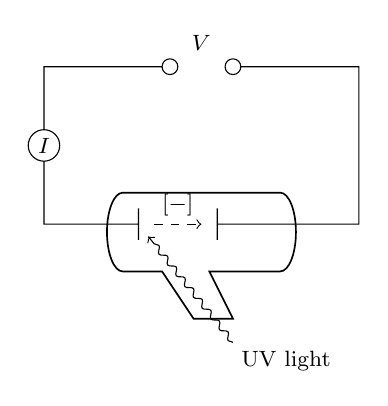
\begin{tikzpicture}
            \footnotesize
            \draw
                (0.4,2) circle (1mm)
                (-0.4,2) circle (1mm)
                (-2,1) circle (2mm) node{$I$}
                (-0.5,2) -- (-2,2) -- (-2,1.2) (-2,0.8) -- (-2,0) -- (-0.8,0) (0.2,0) -- (2,0) -- (2,2) -- (0.5,2)
                (-0.8,-0.2) -- ++(0,0.4) (0.2,-0.2) -- ++(0,0.4)
            ;
            \node at (0,2.3) {$V$};
    
            \draw [semithick] (1,0.4) -- ++(-2,0) arc[start angle=90,end angle=270,x radius=2mm,y radius=5mm] -- ++(0.5,0) -- ++(0.4,-0.6) -- ++(0.5,0) -- ++(-0.3,0.6) -- ++(0.9,0) arc[start angle=-90,end angle=90,x radius=2mm,y radius=5mm];
    
            \draw [decoration={snake,post length=3mm,amplitude=1pt,segment length=5pt},decorate,->,shorten >=2mm] (0.4,-1.5) node[below right]{UV light} -- (-0.8,0);
            \draw [dashed,->] (-0.6,0) -- node[above]{$\e[-]$} (0,0);
        \end{tikzpicture}
        \caption{Photoelectric effect experiment.}
        \label{fig:PEeffectExp}
    \end{figure}
    \begin{itemize}
        \item Shine UV light through a quartz crystal window so that it impinges on the left plate.
        \item This causes an electron to be ejected from the illuminated plate and cross the potential difference (recall that they didn't know about electrons at the time; they just knew something was happening).
        \item Increase the external potential until the spark goes away (gives some data about the energy of the electron).
    \end{itemize}
    \item Odd features:
    \begin{enumerate}
        \item There is a threshold frequency of radiation required to eject the electrons.
        \begin{itemize}
            \item You can shine as much light as you want below a certain frequency and nothing will happen.
            \item However, as soon as you reach that frequency, you get a spark.
        \end{itemize}
        \item The maximum kinetic energy (KE necessary to overcome the voltage PE???) depends linearly upon the frequency and is independent of the intensity.
    \end{enumerate}
    \item Einstein (1906) proposes that light consists of quanta called photons.
    \item If you assume this, Max KE obeys the following form.
    \begin{equation*}
        \frac{1}{2}mv_\text{max}^2 = h\nu-W
    \end{equation*}
    where the work function $W$ is the energy required to remove the photon from the metal.
    \begin{itemize}
        \item When $KE\to 0$, we obtain the threshold frequency
        \begin{equation*}
            \nu_\text{th} = \frac{W}{h}
        \end{equation*}
        required to remove an electron from the metal.
    \end{itemize}
    \item Millikan (1914-1917), hot off the success of the oil drop experiment, experimentally corroborates Einstein's theory at UChicago in Ryerson.
    \begin{itemize}
        \item Noting that $KE=eV$ as well where $e$ is the charge of an electron and $V$ is the stopping voltage, Millikan obtains
        \begin{equation*}
            V = \frac{h}{e}\nu-\frac{W}{e}
        \end{equation*}
        \item The slope of this linear data plot is $h/e$, and Millikan definitely knows the charge of the electron (!), so he can also measure Planck's constant this way.
        \item When Millikan gets the same value Planck got a different way, he corroborates Einstein's theory.
    \end{itemize}
    \item Thus, this quantization is not just one result, but is fundamental to our understanding of radiation.
    \item Bohr (1913) makes assumptions.
    \begin{enumerate}
        \item Circle orbits of electrons about the nucleus.
        \item Only certain stationary orbits are allowed.
        \item The electron radiates energy only during a transition between orbits.
        \item The orbital angular momentum is quantized: $L=\frac{nh}{2\pi}$ where $n\in\N$ is a quantum number.
    \end{enumerate}
    \item Assumption 1 is wrong.
    \item Two equations:
    \begin{itemize}
        \item Equation one: Coulomb attraction of the electron and proton (nucleus) is balanced by a centripetal acceleration.
        \begin{equation*}
            \frac{Ze^2}{4\pi\epsilon_0r^2} = \frac{mv^2}{r}
        \end{equation*}
        where $Z$ is the charge of the nucleus, and $e$ is the charge of an electron.
        \begin{itemize}
            \item This follows exactly from classical mechanics.
        \end{itemize}
        \item Equation two: Quantization of the orbital angular momentum:
        \begin{equation*}
            mvr = \frac{nh}{2\pi} = n\hbar
        \end{equation*}
        where $\hbar=h/2\pi$.
        \begin{itemize}
            \item This is a new development from quantum mechanics.
        \end{itemize}
    \end{itemize}
    \item We now solve the two equations for our two unknowns (the velocity and radius).
    \begin{align*}
        v &= \frac{Ze^2}{4\pi\epsilon_0\hbar n}&
        r &= \frac{4\pi\epsilon_0\hbar^2n^2}{Zme^2}
    \end{align*}
    \item It follows that the translational kinetic energy $T$ is given by
    \begin{align*}
        T &= \frac{1}{2}mv^2\\
        &= \frac{m}{2\hbar}\left( \frac{Ze^2}{4\pi\epsilon_0} \right)^2\frac{1}{n^2}
    \end{align*}
    \begin{itemize}
        \item This is the origin of the $1/n^2$ in the Bohr model.
    \end{itemize}
    \item With respect to potential energy, we also have
    \begin{align*}
        V &= -\frac{Ze^2}{4\pi\epsilon_0r}\\
        &= -\frac{m}{\hbar^2}\left( \frac{Ze^2}{4\pi\epsilon_0} \right)^2\frac{1}{n^2}
    \end{align*}
    \item It follows that the total energy $E$ is given by
    \begin{align*}
        E_n &= T+V\\
        &= -\frac{m}{\hbar^2}\left( \frac{Ze^2}{4\pi\epsilon_0} \right)^2\frac{1}{n^2}
    \end{align*}
    \item Thus, the reason we have discrete transitions is because the atom has discrete energy levels.
    \item Indeed, energy transitions are described by the following.
    \begin{equation*}
        E_b-E_a = hcR_0\left( \frac{1}{n_b^2}-\frac{1}{n_a^2} \right)
    \end{equation*}
    where $R_0$, the Rhydberg constant (observed by Rhydberg and his spectral lines far before Bohr, but applicable here), is all of the other constants swept together.
    \begin{itemize}
        \item Note that
        \begin{equation*}
            R_0 = \frac{m\left( \frac{e^2}{4\pi\epsilon_0} \right)^2}{4\pi c\hbar^3}
        \end{equation*}
        \item Thus, quantum mechanics exactly describes the spectral transitions experimentally described earlier.
    \end{itemize}
    \item Limitations of the Bohr model:
    \begin{enumerate}
        \item Assumption 1.
        \item Cannot be generalized to many electron atoms and models.
        \item No reliable way to predict the time dependence of events like the electron transitions.
    \end{enumerate}
    \item So the Bohr model brings us to the brink of being able to predict chemistry, but we still need to go a bit further.
\end{itemize}



\section{Stern-Gerlach Experiment}
\begin{itemize}
    \item \marginnote{10/1:}Measurement of the magnetic dipole moment of atoms.
    \item Nobel-prize winning experiment done by Otto Stern and W. Gerlach (1922). Stern was Gerlach's grad student.
    \item \textbf{Magnetic dipole moment}: Think about an electron moving in a circle with velocity $v$. Then the charge creates a magnetic field $M$ perpendicular to the plane of the circle.
    \item Thus, we want to detect the magnetic moment of atoms. They will measure this by measuring the deflection of the atoms by an \textbf{inhomogeneous} field.
    \item \textbf{Inhomogeneous} (magnetic field): Because they're not setting up the magnetic field so that its equal everywhere in space through which the beam travels.
    \item They put the atoms in an "oven" to get them hot, and then shoot them through a beam. The beam passes through a magnet, and if the beam has a magnetic moment, it will break up. There is a collection plate at the far end.
    \item Effect of the $\vec{B}$ field: $PE=-\vec{M}\cdot\vec{B}=W$.
    \item It follows that $F=-\nabla W$.
    \item Additionally,
    \begin{equation*}
        F_z = M_z\pdv{B_z}{z}
    \end{equation*}
    \item Classical expectation: Every value of $M_z$ would occur, that is, $|M_z|\leq M$. Would lead to one continuous pile on the collection plate with a Gaussian proportionality.
    \item Stern and Gerlach expect it to be discrete/quantized. Focused on \ce{Ag} atoms. Thought two discrete lines would be formed symmetrically about the center. Thought they would see similar results for \ce{Na}, \ce{Cs}, \ce{K}, \ce{H}.
    \item Didn't see anything at first.
    \item Smoked some cigars, released sulfate, and \ce{AgSO4} (black) showed up on the collection plate in 2 discrete piles.
    \item Bohr quantization (varies from $-\ell$ to $+\ell$, where $\ell$ is orbital angular momentum). $L=\ell\hbar$ (approximately), $L_z=m\hbar$.
    \item Actual quantum mechanics gives us $L=\sqrt{\ell(\ell+1)}\hbar$.
    \item But this does not explain the Stern-Gerlach experiment. According to this theory...
    \begin{itemize}
        \item If $\ell=0$ and $m=0$, then we'll observe just 1 spot.
        \item If $\ell=1$ and $m=-1,0,+1$, then we'll observe 3 spots.
    \end{itemize}
    \item But, of course, they only saw 2 spots.
    \begin{itemize}
        \item The first case corresponds to silver with $\ell=0$.
        \item They were actually seeing electron spin.
    \end{itemize}
    \item Electron spin is later understood by S. Goudsmit and G. E. Uhlenbeck (1925).
    \begin{itemize}
        \item Able to show that the splitting of spectral lines when atoms are placed in $\vec{B}$ fields. The electron must have an intrinsic spin (magnetic moment $M_1$) where two values are allowed: $M_1=\pm\frac{1}{2}$.
        \item They postulate that this is a form of intrinsic angular momentum of spin: $S=\sqrt{s(s+1)}\hbar$.
    \end{itemize}
    \item Total angular momentum: The vector addition of all angular momentum of the part.
    \begin{itemize}
        \item The angular momentum of the nuclei may be neglected. Addition of the orbital and spin angular momentum of the electrons.
    \end{itemize}
    \item Stern and Gerlach:
    \begin{itemize}
        \item The orbital angular momentum of \ce{Ag} atoms is zero.
        \item The net spin angular momentum is $\frac{1}{2}$.
        \item Thus, the total angular momentum $m=\pm\frac{1}{2}$. Thus, we expect two spots on the plate.
    \end{itemize}
    \item Note that this relates to the Pauli exclusion principle (spin implies no more than 2 electrons together), first posited in 1926.
    \item Particle-wave duality (by Louis de Broglie): Introduces matter waves (1923-24).
    \begin{itemize}
        \item Einstein says $E=h\nu$. Additionally, momentum of a photon is $p=h\nu/c=h/\lambda$. Thus, this formula relates the particle (momentum) and wave (wavelength) natures of the photon.
    \end{itemize}
    \item de Broglie: Turns in a 4 page thesis, Paris committee will fail him, but they write to Einstein who recognizes this is really important.
    \begin{itemize}
        \item de Broglie defines a frequency and a wavelength for material particles $\nu=E/h$. It follows that $\lambda=h/p$. Thus, electrons have a wavelength, too.
    \end{itemize}
    \item \textbf{de Broglie's relationship}: The equation
    \begin{equation*}
        \lambda = \frac{h}{mv}
    \end{equation*}
    for a nonrelativistic particle.
    \item Explanation of the Bohr atom:
    \begin{itemize}
        \item For the electron's orbit to be stable, an integer number of wavelengths must match the circumference of the orbit.
        \item This is why the orbits are quantized!
        \item Thus, $n\lambda=2\pi r$ and $L=rp$ (from classical physics), so
        \begin{equation*}
            L = \frac{n\lambda p}{2\pi} = \frac{nh}{2\pi} = n\hbar
        \end{equation*}
        as desired.
    \end{itemize}
\end{itemize}



\section{Chapter 1: The Dawn of the Quantum Theory}
\emph{From \textcite{bib:McQuarrieSimon}.}
\begin{itemize}
    \item \marginnote{9/28:}\textbf{Blackbody}: A body which absorbs and emits all frequencies. \emph{Also known as} \textbf{ideal body}.
    \item "Many theoretical physicists tried to derive expressions consistent with these experimental curves of intensity versus frequency [see Figure \ref{fig:WienLaw1}], but they were all unsuccessful. In fact, the expression that is derived according to the laws of nineteenth century physics is" as follows \parencite[3]{bib:McQuarrieSimon}.
    \item \textbf{Rayleigh-Jeans law}: The equation
    \begin{equation*}
        \dd{\rho(\nu,T)} = \rho_\nu(T)\dd{\nu} = \frac{8\pi k_BT}{c^3}\nu^2\dd{\nu}
    \end{equation*}
    where $\rho_\nu(T)\dd{\nu}$ is the "radiant energy density between the frequencies $\nu$ and $\nu+\dd{\nu}$" \parencite[3]{bib:McQuarrieSimon}.
    \item The ultraviolet catastrophe is so named because the frequency increases as the radiation enters the ultraviolet region.
    \item Planck's solution:
    \begin{itemize}
        \item Rayleigh and Jeans assumed (as does classical physics) that the energies of the electronic oscillators responsible for the emission of the radiation could have any value whatsoever.
        \item However, Planck assumed discrete oscillator energies proportional to an integral multiple of the frequency: $E=nh\nu$, where $n\in\Z$.
        \item Using this quantization energy and ideas from statistical thermodynamics (see Chapter 17), Planck derived the \textbf{Planck distribution law for blackbody radiation}.
        \item The only undetermined constant in the above equation was $h$, and Planck showed that if we let $h=\SI{6.626e-34}{\joule\second}$, then this equation gives excellent agreement with the experimental data for all frequencies and temperatures.
    \end{itemize}
    \item \textbf{Planck distribution law for blackbody radiation}: The equation
    \begin{equation*}
        \dd{\rho(\nu,T)} = \rho_\nu(T)\dd{\nu} = \frac{8\pi h}{c^3}\frac{\nu^3\dd{\nu}}{\e[h\nu/k_BT]-1}
    \end{equation*}
    \begin{itemize}
        \item Note that for small frequencies, the Planck distribution law and Rayleigh-Jeans law converge, but they diverge for large frequencies, as expected.
        \item Because $\nu$ and $\lambda$ are related by $\lambda\nu=c$ (and subsequently by $\dd{\nu}=-c/\lambda^2\dd{\lambda}$), we can write the Planck distribution law in terms of wavelength, as well.
        \begin{equation*}
            \dd{\rho(\lambda,T)} = \rho_\lambda(T)\dd{\lambda} = \frac{8\pi hc}{\lambda^5}\frac{\dd{\lambda}}{\e[hc/\lambda k_BT]-1}
        \end{equation*}
    \end{itemize}
    \item Differentiating $\rho_\lambda(T)$ with respect to $\lambda$ gives an alternate formulation for $b$:
    \begin{equation*}
        \lambda_\text{max}T = \frac{hc}{4.965k_B}
    \end{equation*}
    \item Astronomers use the theory of blackbody radiation to estimate the surface temperatures of stars.
    \begin{itemize}
        \item We can measure the electromagnetic spectrum of a star (which will follow a curve similar to one of the ones in Figure \ref{fig:WienLaw1}).
        \item Then we can find $\lambda_\text{max}$. From here, all that's necessary is to plug into Wien's displacement law:
        \begin{equation*}
            T = \frac{b}{\lambda_\text{max}}
        \end{equation*}
    \end{itemize}
    \item \marginnote{10/3:}\textbf{Photoelectric effect}: The ejection of electrons from the surface of a metal by radiation.
    \item Classical predictions vs. experimental data.
    \begin{itemize}
        \item Classical mechanics: Intensity is proportional to the amplitude squared of the incident light. Thus, the electrons at the surface of the metal should oscillate along with the field, and when they are oscillating violently enough, they should break away from the surface with a kinetic energy that depends on the amplidude/intensity (specifically, \emph{not} the frequency).
        \begin{itemize}
            \item Experimental observation: KE of the ejected electrons is independent of intensity and linearly dependent on the frequency.
        \end{itemize}
        \item Classical mechanics: The photoelectric effect should occur for any frequency of light as long as the intensity is sufficiently high.
        \begin{itemize}
            \item Experimental data: There exists a threshold frequency $\nu_0$, characteristic of the metallic surface, below which no electrons are ejected, regardless of intensity.
        \end{itemize}
    \end{itemize}
    \item \textbf{Work function}: The minimum energy required to remove an electron from the surface of the particular metal. \emph{Denoted by} $\bm{\phi}$. \emph{Units} $\si{\electronvolt}$.
    \begin{itemize}
        \item The work function of the metal is analogous to the ionization energy of an isolated atom.
    \end{itemize}
    \item Bright line spectra: "For many years, scientists had tried to find a pattern in the wavelengths or frequencies of the lines in the hydrogen atom spectrum. Finally, in 1885, an amateur Swiss scientist, Johann Balmer, showed that a plot of the frequency of the lines versus $1/n^2$ ($n=3,4,5,\dots$) is linear" \parencite[10]{bib:McQuarrieSimon}.
    \item \textbf{Balmer's formula}: The equation
    \begin{equation*}
        \tilde{\nu} = \num{109680}\left( \frac{1}{2^2}-\frac{1}{n^2} \right)\si{\per\centi\meter}
    \end{equation*}
    for $n=3,4,5,\dots$, where $\tilde{\nu}$ denotes wavenumber.
    \item \textbf{Balmer series}: The series of lines predicted by Balmer's formula as $n$ takes on the values $3,4,5,\dots$, notably those occurring in the visible and near ultraviolet regions of the hydrogen atomic spectrum.
    \item \textbf{Series limit}: The wavelength of the "last" line in the Balmer series, as $n\to\infty$, of value $\SI{364.7}{\nano\meter}$.
    \item \textbf{Rydberg formula}: The equation
    \begin{equation*}
        \tilde{\nu} = \frac{1}{\lambda} = \num{109680}\left( \frac{1}{n_1^2}-\frac{1}{n_2^2} \right)\si{\per\centi\meter}
    \end{equation*}
    for $n_1,n_2\in\N$ such that $n_2>n_1$.
    \begin{itemize}
        \item The Rydberg formula accounts for all the lines in the hydrogen atomic spectrum.
    \end{itemize}
    \item \textbf{Rydberg constant}: The constant $\SI{109677.57}{\per\centi\meter}$. \emph{Denoted by} $\bm{R_H}$.
    \item The first four series of lines composing the hydrogen atomic spectrum are described in Table \ref{tab:spectralSeriesH}.
    \begin{table}[h!]
        \centering
        \renewcommand{\arraystretch}{1.4}
        \small
        \begin{tabular}{lccl}
            \toprule
            Series name & $n_1$ & $n_2$ & Region of spectrum\\
            \hline
            Lyman   & 1 & $2,3,4,\dots$ & Ultraviolet\\
            Balmer  & 2 & $3,4,5,\dots$ & Visible\\
            Paschen & 3 & $4,5,6,\dots$ & Near infrared\\
            Bracket & 4 & $5,6,7,\dots$ & Infrared\\
            \toprule
        \end{tabular}
        \caption{Hydrogen spectral series.}
        \label{tab:spectralSeriesH}
    \end{table}
    \item Rydberg found approximate empirical laws for many series of lines in many different atoms throughout the 1890s.
    \item \textbf{Ritz combination rule}: The empirical laws for all the observed lines can be expressed as the difference between terms such as those in the Rydberg formula.
    \item \textbf{de Broglie wavelength}: The wavelength $\lambda=h/(mv)$ corresponding to a particle of mass $m$ moving with velocity $v$.
    \item An electron moving at $1.00\%$ the speed of light has a de Broglie wavelength comparable to those of X-rays. Thus, electrons should act like X-rays to an extent.
    \item \textbf{X-ray diffraction}: The scattering of a beam of X-rays directed at a crystalline surface, characteristic of the atomic structure of the crystalline surface.
    \begin{itemize}
        \item Occurs because the interatomic spacings in the crystal are about the same as the wavelength of the X-rays.
    \end{itemize}
    \item The scattering of X-rays and electrons at such crystalline surfaces are very similar.
    \item The wavelike property of electrons is used in electron microscopes.
    \begin{itemize}
        \item "The wavelength of the electrons can be controlled through an applied voltage, and the small de Broglie wavelengths attainable offer a more precise probe than an ordinary light microscope. In addition, in contrast to electromagnetic radiation of similar wavelengths (X-rays and ultraviolet), the electron beam can be readily focused by using electric and magnetic fields, generating sharper images" \parencite[18]{bib:McQuarrieSimon}.
    \end{itemize}
    \item The Bohr model:
    \begin{itemize}
        \item The hydrogen atom has a central, rather massive nucleus with one associated electron. Because the nucleus is so much more massive than the electron, we can approximate it as fixed with the electron revolving around it.
        \item The force $f$ holding the electron in a circular orbit is supplied by the Coulombic force of attraction between the proton and the electron:
        \begin{equation*}
            f = \frac{e^2}{4\pi\epsilon_0r^2}
        \end{equation*}
        \item The Coulombic force is balanced by the centrifugal force
        \begin{equation*}
            f = \frac{m_ev^2}{r}
        \end{equation*}
        \item Since $\sum f_c=0$ for a stable circular orbit, we have
        \begin{equation*}
            \frac{e^2}{4\pi\epsilon_0r^2} = \frac{m_ev^2}{r}
        \end{equation*}
        \item However, according to classical mechanics, an electron under these conditions is constantly accelerating (centripetally), so it should emit EM radiation, lose energy, and spiral into the nucleus. Thus, we make two nonclassical assumptions:
        \begin{enumerate}
            \item Stationary electronic orbits exist.
            \item The de Broglie waves of the orbiting electron must be in phase, as the electron makes one complete revolution.
        \end{enumerate}
        \item For the wave pattern around an orbit to be stable, we must have that the circumference of the orbit is equal to an integral number of wavelengths, i.e.,
        \begin{equation*}
            2\pi r = n\lambda
        \end{equation*}
        where $n\in\N$.
        \item Substituting the de Broglie wavelength formula into the above gives
        \begin{align*}
            2\pi r &= n\cdot\frac{h}{m_ev}\\
            m_evr &= \frac{nh}{2\pi}\\
            m_evr &= n\hbar
        \end{align*}
        where $n\in\N$.
        \begin{itemize}
            \item Since $m_evr$ is the angular momentum of the electron, another interpretation of the above (and the one more commonly attributed to Bohr) is that the angular momentum of the electron about the proton must be quantized.
        \end{itemize}
        \item Solving for $r$ by substituting out $v$ yields
        \begin{equation*}
            r = \frac{\epsilon_0h^2n^2}{\pi m_ee^2}
        \end{equation*}
        \begin{itemize}
            \item Thus, the radii of the allowed \textbf{Bohr orbits} are quantized.
        \end{itemize}
        \item We now consider the total energy of the electron in an atom:
        \begin{align*}
            E &= \text{KE}+V(r)\\
            &= \frac{1}{2}m_ev^2-\frac{e^2}{4\pi\epsilon_0r}\\
            &= \frac{1}{2}\cdot\frac{e^2r}{4\pi\epsilon_0r^2}-\frac{e^2}{4\pi\epsilon_0r}\\
            &= -\frac{e^2}{8\pi\epsilon_0r}\\
            &= -\frac{m_ee^4}{8\epsilon_0^2h^2}\cdot\frac{1}{n^2}
        \end{align*}
        \begin{itemize}
            \item The negative sign in this equation indicates that the energy states are bound states; the energies given are less than when the proton and electron are infinitely separated.
        \end{itemize}
    \end{itemize}
    \item \textbf{First Bohr orbit}: The Bohr orbit corresponding to $n=1$, having radius $\SI{52.92}{\pico\meter}$. \emph{Denoted by} $\bm{a_0}$.
    \item \textbf{Ground state energy}: The lowest energy, corresponding to $n=1$ in the total energy equation.
    \item \textbf{Excited state}: The states of higher energy, i.e., those other than the ground state.
    \begin{itemize}
        \item Generally unstable with respect to the ground state.
        \item At ordinary temperatures, hydrogen atoms as well as other atoms and molecules are found almost exclusively in their ground states.
        \item An atom in an excited state will usually relax back to the ground state and give off the energy as electromagnetic radiation.
    \end{itemize}
    \item With respect to spectral lines, Bohr assumed that the observed spectrum of the hydrogen atom is due to transitions from one allowed energy state to another:
    \begin{equation*}
        \Delta E = \frac{m_ee^4}{8\epsilon_0^2h^2}\left( \frac{1}{n_1^2}-\frac{1}{n_2^2} \right) = h\nu
    \end{equation*}
    \item \textbf{Bohr frequency condition}: The above equation, specifically the relation $\Delta E=h\nu$.
    \begin{itemize}
        \item Implies that as the electron falls from one level to another, the energy evolved is given off as a photon of energy $E=h\nu$.
        \item Making the substitution $h\nu=hc\tilde{\nu}$, we can make the theoretical prediction that spectral lines will be of wavenumber
        \begin{equation*}
            \tilde{\nu} = \frac{m_ee^4}{8\epsilon_0^2ch^3}\left( \frac{1}{n_1^2}-\frac{1}{n_2^2} \right)
        \end{equation*}
        \item It follows that we should have
        \begin{equation*}
            R_\infty = \frac{m_ee^4}{8\epsilon_0^2ch^3}
        \end{equation*}
        which we indeed do.
    \end{itemize}
\end{itemize}




\end{document}